\documentclass[a4paper,11pt]{ctexart}
\usepackage{amsmath}
\usepackage{amssymb}
\usepackage{mathtools}
\usepackage[cdot,amssymb]{SIunits}
\usepackage{graphicx}
\usepackage{hyperref}
\usepackage{verbatim}
\usepackage{braket}

\allowdisplaybreaks

\author{Jiajun Ren \\
\href{mailto:jiajunren0522@gmail.com}{jiajunren0522@gmail.com}}
\title{aggregates Frenkel-Holstein model MPS solver}

\begin{document}
\maketitle
the object of each molecule (mol) has object phonon(ph), each mol has different
number of phonons, omegas, phonon levels, e-ph couplings, localexcitation
energies.

The structure of the MPS/MPO is 
\begin{figure}[htbp]
    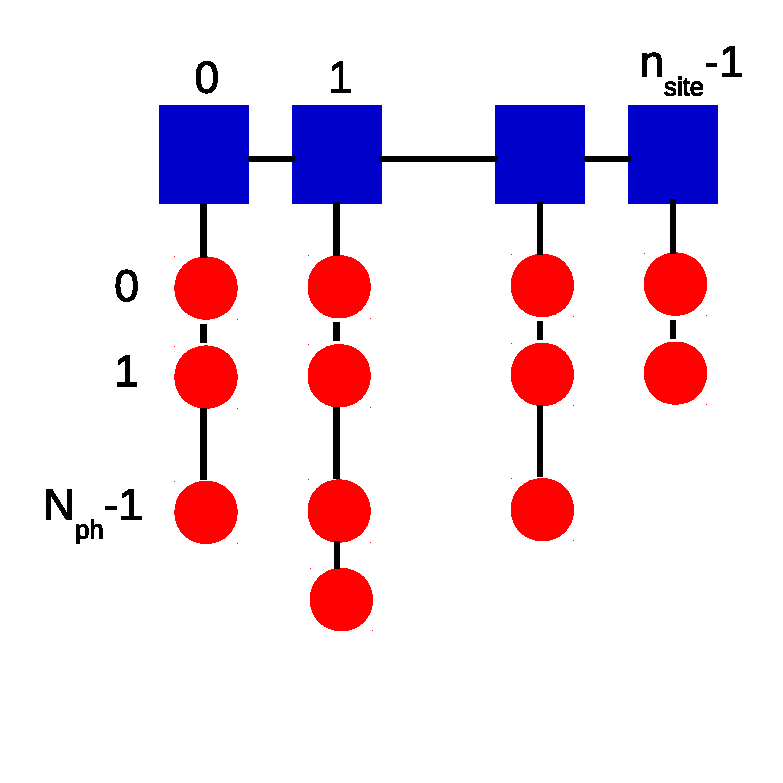
\includegraphics[width = \columnwidth]{structure.eps}  
    \caption{\label{fig:structure} tensor structure }
\end{figure}

\section{MPS structure}
\subsection{eMPS structure}
The eMPS structure is a list [] from mol 0 to mol nsites-1. \\
\# (e physical bond, left bond, right bond, e-ph bond) \\
eMPS(epb, eM, eM, ephM) \\

The eMPSdim is a list[] from 0 to nsites. \\
eMPSdim[0] = eMPSdim[nsites] = 1

\subsection{phMPS structure}
The phMPS structure is a nested list [[],[]] from mol 0 to mol nsites-1. each mol has a
sub list from phonon 0 to nphs-1.\\ (0 index is the left hand site) \\
\# (ph physical bond, left bond, right bond) \\
phMPS(ph.nlevels, phM, phM)
so the leftmost bond is linked to e site e-ph bond

The phMPSdim is a list [] from 0 to mol[imol].nphs
phMPSdim[mol[imol].nphs] = 1
    

\section{MPO structure}
We use the matrix representation to give the MPO
\subsection{eMPO structure}
eMPO is a list from mol 0 to mol nsites-1. \\
\# eMPO(bra, ket, l bond, r bond, e-pb bond)
eMPO(epb,epb,it denpends, it depends, 3)

eMPO structure (lbond, rbond, e-pb bond) is almost a matrix.
The third dimension only has one-line operator to connect phonon part operators.
\begin{gather}
MPO(k) = 
\begin{bmatrix}
    1 & 0 & 0  \\
    A_k & C_k & 0  \\
    B_k & D_k & 1  \\
\end{bmatrix}
\end{gather}

\begin{gather}
A(k) = 
\begin{bmatrix}
    J_{0k} a_k  \\
    J_{0k} a^\dagger_k \\
    ...  \\
    J_{k-1,k} a_k  \\
    J_{k-1,k} a^\dagger_k \\
\end{bmatrix}
\end{gather}

\begin{gather}
B(k) = 
\begin{bmatrix}
    e_k a^\dagger_k a_k \\
\end{bmatrix}
\end{gather}

\begin{gather}
C(k) = 
\begin{bmatrix}
    I & 0 & 0 \\ 
\end{bmatrix}
\end{gather}

\begin{gather}
D(k) = 
\begin{bmatrix}
    0 & ... & 0 & a^\dagger_k & a_k  \\ 
\end{bmatrix}
\end{gather}

remember that the site 0 only has the last row operator,
the site nsites-1 only has the first columnn operator

The third dimenstion linked with phonon part is only attached to $B(k)$
It is 
\begin{gather}
\begin{bmatrix}
    B(k)  \\
    a^\dagger_k a_k \\
    1 \\
\end{bmatrix}
\end{gather}

The eMPOdim is a little bit complicated, because when we move to the right, we
add two operators $a^\dagger_k$ and $a_k$.
The eMPOdim is [1,4,6,8,...,2*nsites,1]
The third dimension is always 3.

\subsection{phMPO structure}
phMPO is a nested list [[]], from mol 0 to mol nsites-1. each mol has sub list
from phonon 0 to phonon nphs-1. 0 index is the left hand site. \\
\# (bra, ket, l bond, rbond)
phMPO(ph.nlevels, ph.nlevels, 3, 3).

The MPO in mol i and phonon n is that: \\
\begin{gather}
MPO(in) = 
\begin{bmatrix}
    1 & 0 & 0  \\
    g_{in} \omega_{in}(b^\dagger_{in}+b_{in}) & 1 & 0  \\
    \omega_{in} b^\dagger_{in}b_{in} & 0 & 1  \\
\end{bmatrix}
\end{gather}
The rightmost MPO has only the first column.
contract these MPOs we finally get
\begin{gather}
MPO(i) = 
\begin{bmatrix}
    1   \\
    \sum_n (g_{in} \omega_{in}(b^\dagger_{in}+b_{in}))   \\
    \sum_n (\omega_{in} b^\dagger_{in}b_{in})  \\
\end{bmatrix}
\end{gather}

The phMPOdim is a list [] from phonon 0 to nphs,
very simple: [3,3,3....,1]

When the temperature is high, then the phonon level should be increased, because
high level phonon excitation is probable. One the other hand, the emission
spectrum is not accurate, because without LF transformation, high level excited
state(high phonon level) is not discribed well, so when they are populated, the
result is probablly wrong. You can see in 1mol1mode, the high level excited
states energy difference is wrong, not the phonon energy


for J aggregates, temperature effect is not so important. the effect temperature
is less than one single molecule.
far side band is not easy to occupied, because the close band density is large
if there is many molecules.

even in the zero temperature, J-aggregates 0-0 is much larger than the 0-1 peak.
Is it due to the addition of the dipole moment?

White's swap algorithm METTS

In the MPSsolver, the left most
\begin{gather}
MPO(1) = 
\begin{bmatrix}
    e_k a^\dagger_k a_k &  a^\dagger_k a_k & a^\dagger_k & a_k & 1 
\end{bmatrix}
\end{gather}

The electronic site MPO is that
\begin{gather}
MPO(k) = 
\begin{bmatrix}
    1 & 0 & 0  \\
    A_k & C_k & 0  \\
    B_k & D_k & 1  \\
\end{bmatrix}
\end{gather}

\begin{gather}
A(k) = 
\begin{bmatrix}
    J_{0k} a_k  \\
    J_{0k} a^\dagger_k \\
    ...  \\
    J_{k-1,k} a_k  \\
    J_{k-1,k} a^\dagger_k \\
\end{bmatrix}
\end{gather}

\begin{gather}
B(k) = 
\begin{bmatrix}
    e_k a^\dagger_k a_k \\
\end{bmatrix}
\end{gather}

\begin{gather}
C(k) = 
\begin{bmatrix}
    0 & I & 0 & 0 \\ 
\end{bmatrix}
\end{gather}

\begin{gather}
D(k) = 
\begin{bmatrix}
    a^\dagger_k a_k & 0 & ... & 0 & a^\dagger_k & a_k  \\ 
\end{bmatrix}
\end{gather}

The phonon site MPO is that
\begin{gather}
A(k) = 
\begin{bmatrix}
    g_{in} \omega_{in}(b^\dagger_{in}+b_{in})  \\
    0 \\
    0 \\
\end{bmatrix}
\end{gather}

\begin{gather}
B(k) = 
\begin{bmatrix}
    \omega_{in} b^\dagger_{in}b_{in}   \\
\end{bmatrix}
\end{gather}

\begin{gather}
C(k) = 
\begin{bmatrix}
    I \\ 
\end{bmatrix}
\end{gather}

\begin{gather}
D(k) = 
\begin{bmatrix}
     0 \\ 
\end{bmatrix}
\end{gather}

the right most phonon is that
\begin{gather}
C(k) = 
\begin{bmatrix}
    0 \\
    I \\ 
\end{bmatrix}
\end{gather}

时间步长的确定应该有两个标准,
一个是对最后光谱的精确性要求,因为信号的频率太大,那么就要求时间的间隔要很小,解
决这个的办法是H-H0,这样相当于先抽出已知光谱中的高频的部分,做一个整体的平移,剩
下的低频的部分,就可以用时间间隔比较大的来采样。同样的omega部分的分辨率,那么步
数就会少,计算量就小。

当时这是建立在每一个时间点都能算对的情况下。这就是另外一个对时间步长的要求,即每
个点都要算对。在Runge-Kutta下,时间步长不能太大,即使已经做了H-H0。对H做一个
scale是没用的,因为H是小了,t是大了,但是omega部分的分辨率要求也高了,所以要求整个步数
没变,计算量没变。这一点可以从发射光谱的精确演化和Rungekutta的步长看出来。精确演
化,$e^iHt$,每一步都是精确的,但是Runge-kutta他总是按照(1-iHt)变得化总是有误差
。

In the zero temperature case, the time correlaiton function we calculate is that
\begin{gather}
    \langle i | e^{iHt} \hat{A} e^{-iHt} \hat{A} | i \rangle 
    = e^{iE_{i0} t} \langle \hat{A}i | e^{-iHt} | \hat{A} i \rangle 
    = e^{i(E_{i0}-E_{f0}) t} \langle \hat{A}i | e^{-i(H-E_{f0})t} | \hat{A} i \rangle
\end{gather}
if FFT the whole expression, then the exact pole should be
$\omega_{exact} = E_{f0}-E_{fm} + E_{i0}-E_{f0}$
if FFT the braket part, the calculated pole is 
$\omega_{calc} = E_{f0}-E_{fm}$
so the recover final result should be 
$\omega_{exact} = \omega_{calc} + E_{i0}-E_{f0}$


\section{calculate the finite temperature dynamic property}
We use the so-called purification method.
In principle, the mixed states density operator can be expressed as a enlarged
space pure state density operator by trace out the enviroment
\begin{gather}
    \sum_i s_i | i \rangle \langle i | = \textrm{Tr}_Q  | \Psi \rangle \langle \Psi |
\end{gather}
$\Psi$ can be expressed as (many expression, because P,Q space rotation do not
change it)
\begin{gather}
    | \Psi \rangle =  \sum_i s_i^{1/2} | i \rangle_P | i \rangle_Q 
\end{gather}


So, the density operator is 
\begin{gather}
    \frac{e^{-\beta \hat{H}}}{Z(\beta)} = \frac{1}{Z(\beta)} e^{-\beta
    \hat{H}/2} \hat{I}  e^{-\beta \hat{H}/2}
\end{gather}
The identity operator can be expressed as reduced density
operator of a maximum entangled state $| \Psi \rangle$ at $T=\infty$
\begin{gather}
    \hat{I} = \sum_i | i \rangle \langle i | = N \sum_{i=1}^N  \frac{1}{N} | i
    \rangle \langle i | = Z(0) \textrm{Tr}_Q | \Psi \rangle \langle \Psi |
\end{gather}

So, 
\begin{gather}
    \frac{e^{-\beta \hat{H}}}{Z(\beta)} = \frac{Z(0)}{Z(\beta)} \textrm{Tr}_Q
    e^{-\beta \hat{H}/2}| \Psi \rangle \langle \Psi |e^{-\beta \hat{H}/2} 
\end{gather}

Since
\begin{gather}
    \textrm{Tr}_P\frac{e^{-\beta \hat{H}}}{Z(\beta)} = 1
\end{gather}
So, 
\begin{gather}
    \frac{Z(\beta)}{Z(0)} = \langle \Psi | e^{-\beta \hat{H}} | \Psi
    \rangle  
\end{gather}

So, the dynamic correlaiton function is that
\begin{gather}
    \textrm{Tr}_P \frac{e^{-\beta \hat{H}}}{Z(\beta)} e^{i\hat{H}t} \hat{A}
    e^{-i\hat{H}t} \hat{A} =  \frac{
    \langle \Psi | e^{-\beta \hat{H} /2 } e^{i\hat{H}t} \hat{A} e^{-i\hat{H}t}
    \hat{A}
   e^{-\beta \hat{H} /2 } | \Psi \rangle  }{\langle \Psi | e^{-\beta \hat{H}} | \Psi \rangle}
\end{gather}

\begin{gather}
    | \Psi \rangle = \sum_{i=1}^n \frac{1}{\sqrt{n}} |i\rangle_P |i\rangle_Q
\end{gather}

$\Psi$ is the initial maximum correlated state in a enlarged space. It is
actually a MPO, but only when the up and down physical bond index equals the MPO
is nonzero, when nonequal, it is zeros.

The GS state is very simple, the bond dimension is 1. electron site is 0 when
physical index is 1, 1 when physical index is 0. The phonon site is 1.

The EX state is a little bit complicated, we can imagine applying a operator
$\sum_i a^\dagger_i$ to a GS maximum correlation state, so the bond dimension is
2 at most.

For the 0T abs case, we use two different algorithms to calculate the
correlation function. One is only propagating the ket, the other is propagating
the ket and bra the same time. The second one is more accurate with same bond
dimension, because the ket and bra are both huge correlated, MPS take effect in
both bra and ket. The first one only ket MPS take effect. The bra takes less
effect.
1. Nstep: 0, dt, 2dt ... Nsteps*dt
2. -Nsteps/2*dt,...0,... Nsteps/2, the negative part propagator in bra, positive
part propagator in ket.

because of the commucate between dipole operator and GS state H.

if emi:
\begin{gather}
    \textrm{Tr}_P \frac{e^{-\beta \hat{H}}}{Z(\beta)} e^{i\hat{H}t} \hat{A}
    e^{-i\hat{H}t} \hat{A} =  \frac{
        \langle \Psi | e^{-\beta \hat{H}_{EX} /2 } e^{i\hat{H}_{EX}t}
        e^{-i\hat{H}_{GS}t} \hat{A} 
    \hat{A}
    e^{-\beta \hat{H}_{EX} /2 } | \Psi \rangle  }{\langle \Psi | e^{-\beta \hat{H}} | \Psi \rangle}
\end{gather}

if abs:
\begin{gather}
    \textrm{Tr}_P \frac{e^{-\beta \hat{H}}}{Z(\beta)} e^{i\hat{H}t} \hat{A}
    e^{-i\hat{H}t} \hat{A} =  \frac{
        \langle \Psi | e^{-\beta \hat{H}_{GS} /2 } \hat{A} e^{i\hat{H}_{GS}t}
        e^{-i\hat{H}_{EX}t}
    \hat{A}
    e^{-\beta \hat{H}_{GS} /2 } | \Psi \rangle  }{\langle \Psi | e^{-\beta \hat{H}} | \Psi \rangle}
\end{gather}
when considering propagating both sides of the bra and ket, only emission is
probable:
\begin{gather}
    \textrm{Tr}_P \frac{e^{-\beta \hat{H}}}{Z(\beta)} e^{i\hat{H}t} \hat{A}
    e^{-i\hat{H}t} \hat{A} =  \frac{
        \langle \Psi | e^{-\beta \hat{H}_{EX} /2 } e^{i\hat{H}_{EX}t/2}
        \hat{A} e^{-i\hat{H}_{GS}t}  
    \hat{A} e^{i\hat{H}_{EX}t/2}
    e^{-\beta \hat{H}_{EX} /2 } | \Psi \rangle  }{\langle \Psi | e^{-\beta \hat{H}} | \Psi \rangle}
\end{gather}


\end{document}
